\chapter{UNIXシェル}
本章では簡易版のUNIXシェル(以下では myshell\footnote{
\url{https://raw.githubusercontent.com/tctsigemura/SystemPrograming/master/myshell.c}
}と呼ぶ)を紹介する.
これの内容を理解し,更に,改造したりすることで,
「fork-exec方式」,
「環境変数」,
「リダイレクト」等の理解を深める.
最後の課題で,
myshellに幾つかの機能を追加できるようになることを目標とする.

%=============================================================================
\section{UNIXのシェルとは}
UNIXのシェルはCLI(Command Line Interface)方式の
コマンドインタプリタ\footnote{
macOSのFinderや,WindowsのExplorerはGUI版のシェルである.}である.
UNIX,Linux,macOS,WSL(Windows Subsystem for Linux)等で使用される.
ユーザが入力したコマンド行を解析し実行する.
またコマンド行だけではなく,
コマンド列(シェルスクリプト)を書いたファイルを実行する機能も備えており,
処理の自動化にも役立つ.
実際にUNIX系OSの多くでは,
システム起動時に自動的にサービスを立ち上げる等の処理に,
シェルスクリプトが多用されている.
\ref{environment}章で紹介した\|/etc/zprofile|や\|.zprofile|も
シェルスクリプトの一種である.

シェルはユーザプログラムの一種であり,
ユーザプロセスとして実行される.
macOSでは\|sh|,\|bash|,\|ksh|,\|zsh|,\|csh|,\|tcsh|等,
多種類のUNIXのシェルが予めインストールされており利用可能である.
macOSの場合,標準のログインシェル\footnote{
ターミナルを開いたとき最初に使用されるシェルのこと.
}は\|zsh|になっているが,好みで変更する\footnote{
chshコマンドで変更する.}ことも可能である.
% これらのUNIXシェルはどれも高機能なものであり,
% かなり大きなプログラムである.
UNIXシェルは最低でも次の機能を持っている.

\begin{enumerate}
\item 外部コマンド(プログラム)を起動する機能
\item カレントディレクトリを変更する機能
\item 環境変数などの変数管理機能
\item 入出力のリダイレクト機能やパイプ機能(\|<|,\|>|,\|>>|,\verb;|;)
\item ジョブ制御機能(jobs,fg,bg,\|&|,\|;|など)
\item ファイル名の展開機能(ワイルドカード)
\item 繰り返しや条件判断機能
\item スクリプトの実行機能(処理の自動化)
\end{enumerate}

%=============================================================================
\section{簡易UNIXシェル(myshell)}
myshellはC言語で70行以内で記述可能な簡易版UNIXシェルである.
ここでは,シェルの仕組みを理解するための教材として用いる.
コマンド行は空白区切りの文字列とする.
myshellは以下の二つの機能しか持たない.

\begin{enumerate}
\item 外部コマンド(プログラム)を起動する機能
\item カレントディレクトリを変更する機能
\end{enumerate}

\subsection{基本構造(\texttt{main()}関数)}
myshell は,コマンド行の\emph{入力},\emph{解析},\emph{実行}を
入力がEOFになるまで繰り返す.
これを,リスト\ref{myshellMain}の\|main()|関数で行う.
\|main()|関数の動作は次の通りである.

\lstinputlisting[label=myshellMain
  ,caption=メインループ(\texttt{main()})
  ,float=btp, numbers=left, firstline=46, lastline=66]{Lst/myshell.c}

\begin{enumerate}
\item 6行で
  \|fgets()|関数\footnote{
    \texttt{fgets()}関数はC言語の標準ライブラリ関数である.
  }を用いてコマンド行を\|buf|配列に\emph{入力}する.
  \|buf|配列には\|'\n'|,\|'\0'|で終端された文字列が格納されるはずである.
\item 10行では,
  \|strchr()|関数\footnote{
    \texttt{strchr()}関数はC言語の標準ライブラリ関数である.
  }を用いてバッファに\|'\n'|が格納されていることを確認する.
  格納されていない場合は,
  「コマンド行が長すぎてバッファに入り切らない」エラーが発生した場合である.
  簡易版のシェルなのでエラーからの復旧は諦めて,
  エラーメッセージを表示し終了する.
\item 14行では,
  後で説明する\|parse()|関数を用いて\|buf|配列のコマンド行を\emph{解析}し,
  execveシステムコールに渡す\|args|配列を作る.
  もしも,コマンド行の文字列が多すぎて配列に格納しきれない時は,
  \|parse()|関数が\|0|を返すのでエラーメッセージを表示して入力を無視する.
\item 18行では,
  \|args|配列にコマンドが格納されていることを確認した後,
  後で説明する\|execute()|関数に依頼して
  \|args|配列のコマンドを\emph{実行}する.
\end{enumerate}

\subsection{コマンド行の解析(\texttt{parse()}関数)}
\|parse()|関数がコマンド行を解析し\|execve()|システムコールの
第2引数で使用できる\|argv|形式に変換する.
リスト\ref{myshellParse}にmyshellの\|parse()|関数を示す.
動作は次の通りである.

\lstinputlisting[label=myshellParse
  ,caption=コマンド行の解析ルーチン(\texttt{parse()})
  ,float=btp, numbers=left, firstline=10, lastline=20]{Lst/myshell.c}

\begin{enumerate}
\item コマンド行に入力された文字列と,
  解析結果を格納する文字列配列を引数に呼出される.
\item 4行では,
  \|isspace()|関数\footnote{
    \texttt{isspace()}関数は空白文字を判定するC言語の標準ライブラリ関数である.
    スペース,タブ,改行などを空白と判定する.
  }を用いて文字列に先行する空白を読み飛ばす(ポインタ\|p|を進める).
  その際,空白を文字列の終端記号である\|'\0'|に置き換えておく.
\item 5行では,解析処理の完了を判断する.
  空白を読み飛ばした後で最初に見つかった文字が\|'\0'|なら,
  コマンド行の最後まで達しているので\|for(;;)|ループを脱出し解析を終了する.
  または,\|args|配列のサイズを超えそうになっていた場合も,
  文字列が多すぎてこれ以上処理できないのでループを終了する.
% この時は12行でエラーを意味する\|0|(false)を返す.
\item 処理が6行に進むのは,
  新しく次の文字列が見つかった場合である.
  新しい文字列の開始位置(ポインタ)を\|args|配列に記録する.
\item 7行では,\|isspace()|関数を用いて文字列を終端する空白を探す.
  終端が見つかったら\|for(;;)|ループの先頭に戻り,
  4行で空白を\|'\0'|に書換えC言語の文字列として完成する.
\item 9,10行では,
  文字列配列に配列の終端を表す\|NULL|を書込み\|parse()|関数を終了する.
  その際,コマンド行の最後まで解析が終わっていれば\|1|(true)を,
  そうでなければ\|0|(false)を返す.
\end{enumerate}

\begin{myfig}{btp}{\texttt{parse()}関数の実行結果例}{myshellArgs}
  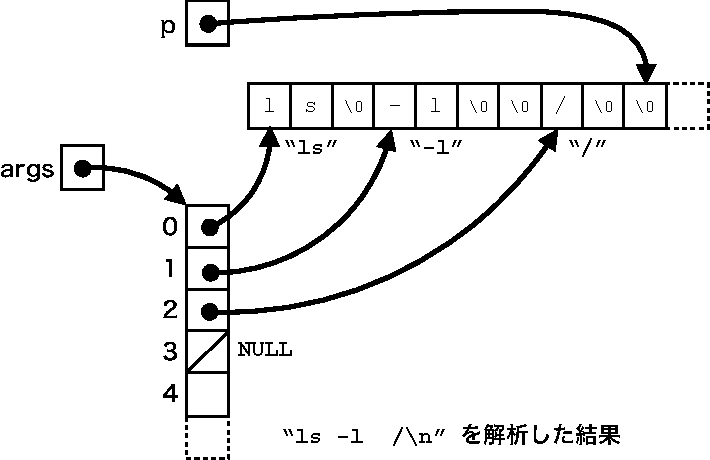
\includegraphics[scale=0.8]{Fig/myshellArgs-crop.pdf}
\end{myfig}

\figref{myshellArgs}に\|parse()|関数実行後のデータ構造の例を示す.
この例は,コマンド行文字列
~\texttt{"ls{\textvisiblespace}-l{\textvisiblespace}{\textvisiblespace}/{\bs}n"}~
を解析した後のデータ構造である.
渡された文字列の空白を\|'\0'|で上書きし
\|"ls"|,\|"-l"|,\|"/"|の3つの文字列が作られている\footnote{
  リスト\ref{myshellParse}の4行で\texttt{'{\bs}0'}に書換えている.}.
文字列配列の終端は\|NULL|で表現する.
\|args|配列は各文字列の先頭を指すポインタを格納する\footnote{
  リスト\ref{myshellParse}の6行でポインタを\texttt{args}配列に格納している.
}ことで文字列配列を表現する.
文字列の最後の \|'\n'| は \|'\0'| に書き換わっている\footnote{
  \texttt{'{\bs}n'}は\texttt{isspace()}関数により空白と判断される.
}.

\subsection{コマンドの実行(\texttt{execute()})}
リスト\ref{myshellExecute}にmyshellの\|execute()|関数を示す.
この関数は\|parse()|関数が作った\|args|配列を受け取り,
内部コマンドなら自分で実行し,
外部コマンドなら子プロセスを作って実行させる.

\lstinputlisting[label=myshellExecute
  ,caption=コマンドの実行ルーチン(\texttt{execute()})
  ,float=btp, numbers=left, firstline=22, lastline=44]{Lst/myshell.c}

2行ではコマンドの名前を調べている.
cd コマンドは内部コマンドなので,
5行で自ら\|chdir()|システムコールを実行している\footnote{
  内部コマンドを追加するときは,cd コマンドと同様に,ここに追加する.}.
8行以下は外部コマンドの処理である.
10行で子プロセスを作り,15行で子プロセスがコマンドを実行する.
親プロセスは19行で子プロセスの終了を待つ.

15行では\|execve()|システムコールの代わりに\|execvp()|関数を用いているので,
PATH環境変数を用いたプログラムの自動的な探索が行われる.

%=============================================================================
%\newpage
%\section*{課題 No.11}
%
%\begin{enumerate}
%\item myshell に環境変数を追加するコマンド setenv ,
%  削除するコマンド unsetenv を追加しなさい.
%\item myshell にリダイレクト機能を追加しなさい.
%\end{enumerate}
%
%\subsection*{機能追加後のmyshellの実行例(参考)}
%\begin{lstlisting}[numbers=none]
%Command: setenv A B
%Command: printenv A
%B
%Command: unsetenv A
%Command: printenv A
%Command: echo aaa > a.txt
%Command: cat a.txt
%aaa
%Command:
%\end{lstlisting}
